%%%%%%%%%%%%%%%%%%%%%%%%%%%%%%%%%%%%%%%%%
% Template
% LaTeX Template
% Version 1.0 (December 8 2014)
%
% This template has been downloaded from:
% http://www.LaTeXTemplates.com
%
% Original author:
% Brandon Fryslie
% With extensive modifications by:
% Vel (vel@latextemplates.com)
%
% License:
% CC BY-NC-SA 3.0 (http://creativecommons.org/licenses/by-nc-sa/3.0/)
%
% Authors:
% Sabbir Ahmed
% 
%%%%%%%%%%%%%%%%%%%%%%%%%%%%%%%%%%%%%%%%%

\documentclass[paper=usletter, fontsize=12pt]{article}
%%%%%%%%%%%%%%%%%%%%%%%%%%%%%%%%%%%%%%%%%
% Contract Structural Definitions File Version 1.0 (December 8 2014)
%
% Created by: Vel (vel@latextemplates.com)
% 
% This file has been downloaded from: http://www.LaTeXTemplates.com
%
% License: CC BY-NC-SA 3.0 (http://creativecommons.org/licenses/by-nc-sa/3.0/)
%
%%%%%%%%%%%%%%%%%%%%%%%%%%%%%%%%%%%%%%%%%

\usepackage{geometry} % Required to modify the page layout
\usepackage{multicol}
\usepackage{amsmath}
\usepackage{amssymb}

\usepackage[pdftex]{graphicx}
\usepackage{wrapfig}
\usepackage[font=scriptsize, labelfont=bf]{caption}
\usepackage[utf8]{inputenc} % Required for including letters with accents
\usepackage[T1]{fontenc} % Use 8-bit encoding that has 256 glyphs

\usepackage{avant} % Use the Avantgarde font for headings
\usepackage{courier}
\usepackage{xparse}
\usepackage{xcolor}
\usepackage{listings}  % for code verbatim and console outputs

\setlength{\textwidth}{16cm} % Width of the text on the page
\setlength{\textheight}{23cm} % Height of the text on the page
\setlength{\oddsidemargin}{0cm} % Width of the margin - negative to move text left, positive to move it right
\setlength{\topmargin}{-1.25cm} % Reduce the top margin

\setlength{\parindent}{0mm} % Don't indent paragraphs
\setlength{\parskip}{2.5mm} % Whitespace between paragraphs
\renewcommand{\baselinestretch}{1.5}

\definecolor{green}{rgb}{0.18, 0.55, 0.34}

\graphicspath{ {figures/} }
\captionsetup[table]{skip=10pt}

\lstset{language=C, keywordstyle={\bfseries \color{black}}}

% defines algorithm counter for chapter-level
\newcounter{nalg}[section]

%defines appearance of the algorithm counter
\renewcommand{\thenalg}{\thesection .\arabic{nalg}}

% defines a new caption label as Algorithm x.y
\DeclareCaptionLabelFormat{algocaption}{Algorithm \thenalg}

% defines the algorithm listing environment
\lstnewenvironment{pseudocode}[1][] {
    \refstepcounter{nalg}  % increments algorithm number
    \captionsetup{font=normalsize, labelformat=algocaption, labelsep=colon}
    \lstset{
        breaklines=true,
        mathescape=true,
        numbers=left,
        numberstyle=\scriptsize,
        basicstyle=\footnotesize\ttfamily,
        keywordstyle=\color{black}\bfseries,
        keywords={input, output, return, parallel, function, for, to, in, if,
        else, foreach, while, and, or, new, print},
        xleftmargin=.04\textwidth,
        #1
    }
}{}

\renewcommand{\familydefault}{\sfdefault}  % default font for entire document
 % specifies the document layout and style

\begin{document}

    \documentinfo{\textbf{Question:} 06}{\textbf{DATE:} \today}{Sabbir Ahmed}
    \vspace{-0.1in}

    \section{Background}
    Add \textbf{\$display} calls to the above code after every assignment statement and resimulate to show that multiple assignments are observable in simulation whereas \textbf{\$strobe} only prints one final result per change event. Both your \textbf{\$display} and \textbf{\$strobe} calls should print time using \%0t and \textbf{\$time}.

    \section{Implementation}
    The provided code was directly used to implement the module in Part 7, and can be found in the `scripts' directory. \textbf{\$display} statements were added after each assignment statements in the module.

    A sample of the waveform generated is provided:

    \begin{figure}[ht]
        \begin{center}
            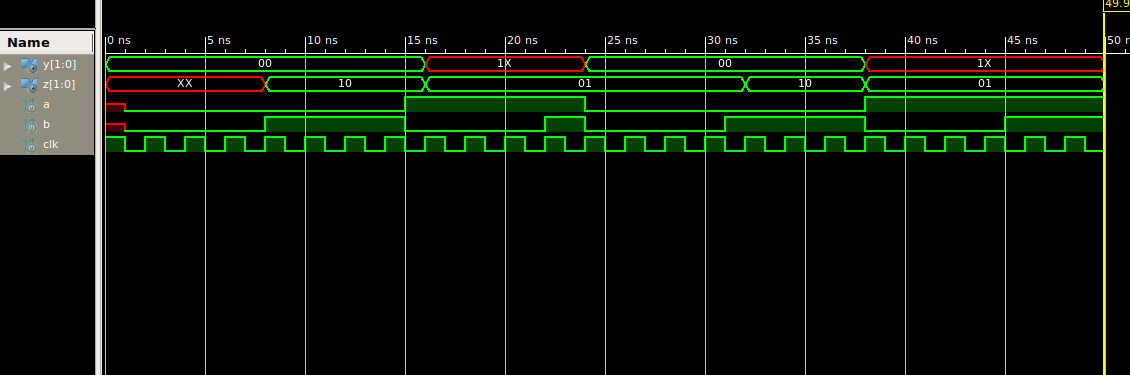
\includegraphics[width=1\textwidth]{wav.png}
            \caption{Waveform Generated from Part 7 Test Bench} \label{fig:wav}
        \end{center}
    \end{figure}

    The following output is dumped from the test bench as well, demonstrating the difference in the usage of \textbf{\$display}:

    The following table is generated from the test bench as well, demonstrating the usage of the circuit:

    \begin{longtable*}{@{\extracolsep{\fill}} ccccc}

        \textbf{time} & \textbf{a} & \textbf{b} & \textbf{y} & \textbf{z} \\
        \hline
        2000 & 0 & 0 & 00 & xx \\
        3000 & 0 & 0 & 00 & xx \\
        4000 & 0 & 0 & 00 & xx \\
        6000 & 0 & 0 & 00 & xx \\
        8000 & 0 & 1 & 00 & xx \\
        8000 & 0 & 1 & 00 & xx \\
        8000 & 0 & 1 & 00 & xx \\
        8000 & 0 & 1 & 00 & 10 \\
        10000 & 0 & 1 & 00 & 10 \\
        10000 & 0 & 1 & 00 & 10 \\
        10000 & 0 & 1 & 00 & 10 \\
        10000 & 0 & 1 & 00 & 10 \\
        10000 & 0 & 1 & 00 & 10 \\
        12000 & 0 & 1 & 00 & 10 \\
        12000 & 0 & 1 & 00 & 10 \\
        12000 & 0 & 1 & 00 & 10 \\
        12000 & 0 & 1 & 00 & 10 \\
        14000 & 0 & 1 & 00 & 10 \\
        14000 & 0 & 1 & 00 & 10 \\
        14000 & 0 & 1 & 00 & 10 \\
        14000 & 0 & 1 & 00 & 10 \\
        16000 & 1 & 0 & 00 & 10 \\
        16000 & 1 & 0 & 10 & 10 \\
        16000 & 1 & 0 & 1x & 10 \\
        16000 & 1 & 0 & 1x & 01 \\
        17000 & 1 & 0 & 1x & 01 \\
        18000 & 1 & 0 & 00 & 01 \\
        18000 & 1 & 0 & 10 & 01 \\
        18000 & 1 & 0 & 1x & 01 \\
        18000 & 1 & 0 & 1x & 01 \\
        20000 & 1 & 0 & 00 & 01 \\
        20000 & 1 & 0 & 10 & 01 \\
        20000 & 1 & 0 & 1x & 01 \\
        20000 & 1 & 0 & 1x & 01 \\
        22000 & 1 & 1 & 00 & 01 \\
        22000 & 1 & 1 & 10 & 01 \\
        22000 & 1 & 1 & 1x & 01 \\
        22000 & 1 & 1 & 1x & 01 \\
        24000 & 0 & 0 & 00 & 01 \\
        24000 & 0 & 0 & 00 & 01 \\
        26000 & 0 & 0 & 00 & 01 \\
        26000 & 0 & 0 & 00 & 01 \\
        28000 & 0 & 0 & 00 & 01 \\
        30000 & 0 & 0 & 00 & 01 \\
        32000 & 0 & 1 & 00 & 01 \\
        32000 & 0 & 1 & 00 & 01 \\
        32000 & 0 & 1 & 00 & 01 \\
        32000 & 0 & 1 & 00 & 10 \\
        33000 & 0 & 1 & 00 & 10 \\
        34000 & 0 & 1 & 00 & 10 \\
        34000 & 0 & 1 & 00 & 10 \\
        34000 & 0 & 1 & 00 & 10 \\
        34000 & 0 & 1 & 00 & 10 \\
        36000 & 0 & 1 & 00 & 10 \\
        36000 & 0 & 1 & 00 & 10 \\
        36000 & 0 & 1 & 00 & 10 \\
        36000 & 0 & 1 & 00 & 10 \\
        38000 & 1 & 0 & 00 & 10 \\
        38000 & 1 & 0 & 10 & 10 \\
        38000 & 1 & 0 & 1x & 10 \\
        38000 & 1 & 0 & 1x & 01 \\
        40000 & 1 & 0 & 00 & 01 \\
        40000 & 1 & 0 & 10 & 01 \\
        40000 & 1 & 0 & 1x & 01 \\
        40000 & 1 & 0 & 1x & 01 \\
        40000 & 1 & 0 & 1x & 01 \\
        42000 & 1 & 0 & 00 & 01 \\
        42000 & 1 & 0 & 10 & 01 \\
        42000 & 1 & 0 & 1x & 01 \\
        42000 & 1 & 0 & 1x & 01 \\
        44000 & 1 & 0 & 00 & 01 \\
        44000 & 1 & 0 & 10 & 01 \\
        44000 & 1 & 0 & 1x & 01 \\
        44000 & 1 & 0 & 1x & 01 \\
        46000 & 1 & 1 & 00 & 01 \\
        46000 & 1 & 1 & 10 & 01 \\
        46000 & 1 & 1 & 1x & 01 \\
        46000 & 1 & 1 & 1x & 01 \\
        47000 & 1 & 1 & 1x & 01 \\
        48000 & 1 & 1 & 00 & 01 \\
        48000 & 1 & 1 & 10 & 01 \\
        48000 & 1 & 1 & 1x & 01 \\
        48000 & 1 & 1 & 1x & 01 \\
    \end{longtable*}

    \section{Observations}
    The addition of \textbf{\$display} obviously generates a greater amount of output, where it outputs when it notices change in any variables.

\end{document}
